\documentclass[a4paper,12pt]{article}
\usepackage[utf8]{inputenc}
\usepackage[margin=1in]{geometry}
\usepackage{parskip}
\usepackage{graphicx}
\usepackage{hyperref}
\usepackage{listings}
\usepackage{multirow}
\hypersetup{colorlinks}
\lstset{basicstyle=\ttfamily}

\title{Data Structures and Algorithms 120:\\Inventory Assignment Report}
\date{October 7, 2013}
\author{Delan Azabani}

\begin{document}

\maketitle

\pagenumbering{arabic}

\section{Known defects}

The application allows the user to build a binary search tree regardless of
whether or not the array has been sorted due to the invocation of the ``Save
data to file'' function. Doing so after the data is output to a file will cause
a degenerate tree to be built, which is extremely inefficient. I chose not to
manually prevent this to allow a live comparison of the two scenarios,
demonstrating the importance of using a randomised input array.

\section{Duplicate keys in the binary search tree}

When faced with unknown data from an external input file, there is a chance
that the given data may contain tuples with duplicate keys, which does not make
sense when the key is used as a \emph{unique} identifier. An implementation of
this assignment could throw an exception when faced with a duplicate key and
stop processing the input file altogether, or ignore the bad row and continue
with the rest of the file.

I have decided to take the latter, more resilient approach to handling
duplicate keys, as well as any other line parsing errors. While bst.insert()
throws an IllegalArgumentException, this is caught by the caller, counted as a
failed line by its caller, and the remainder of the input file continues to be
processed.

\section{UML class diagram}

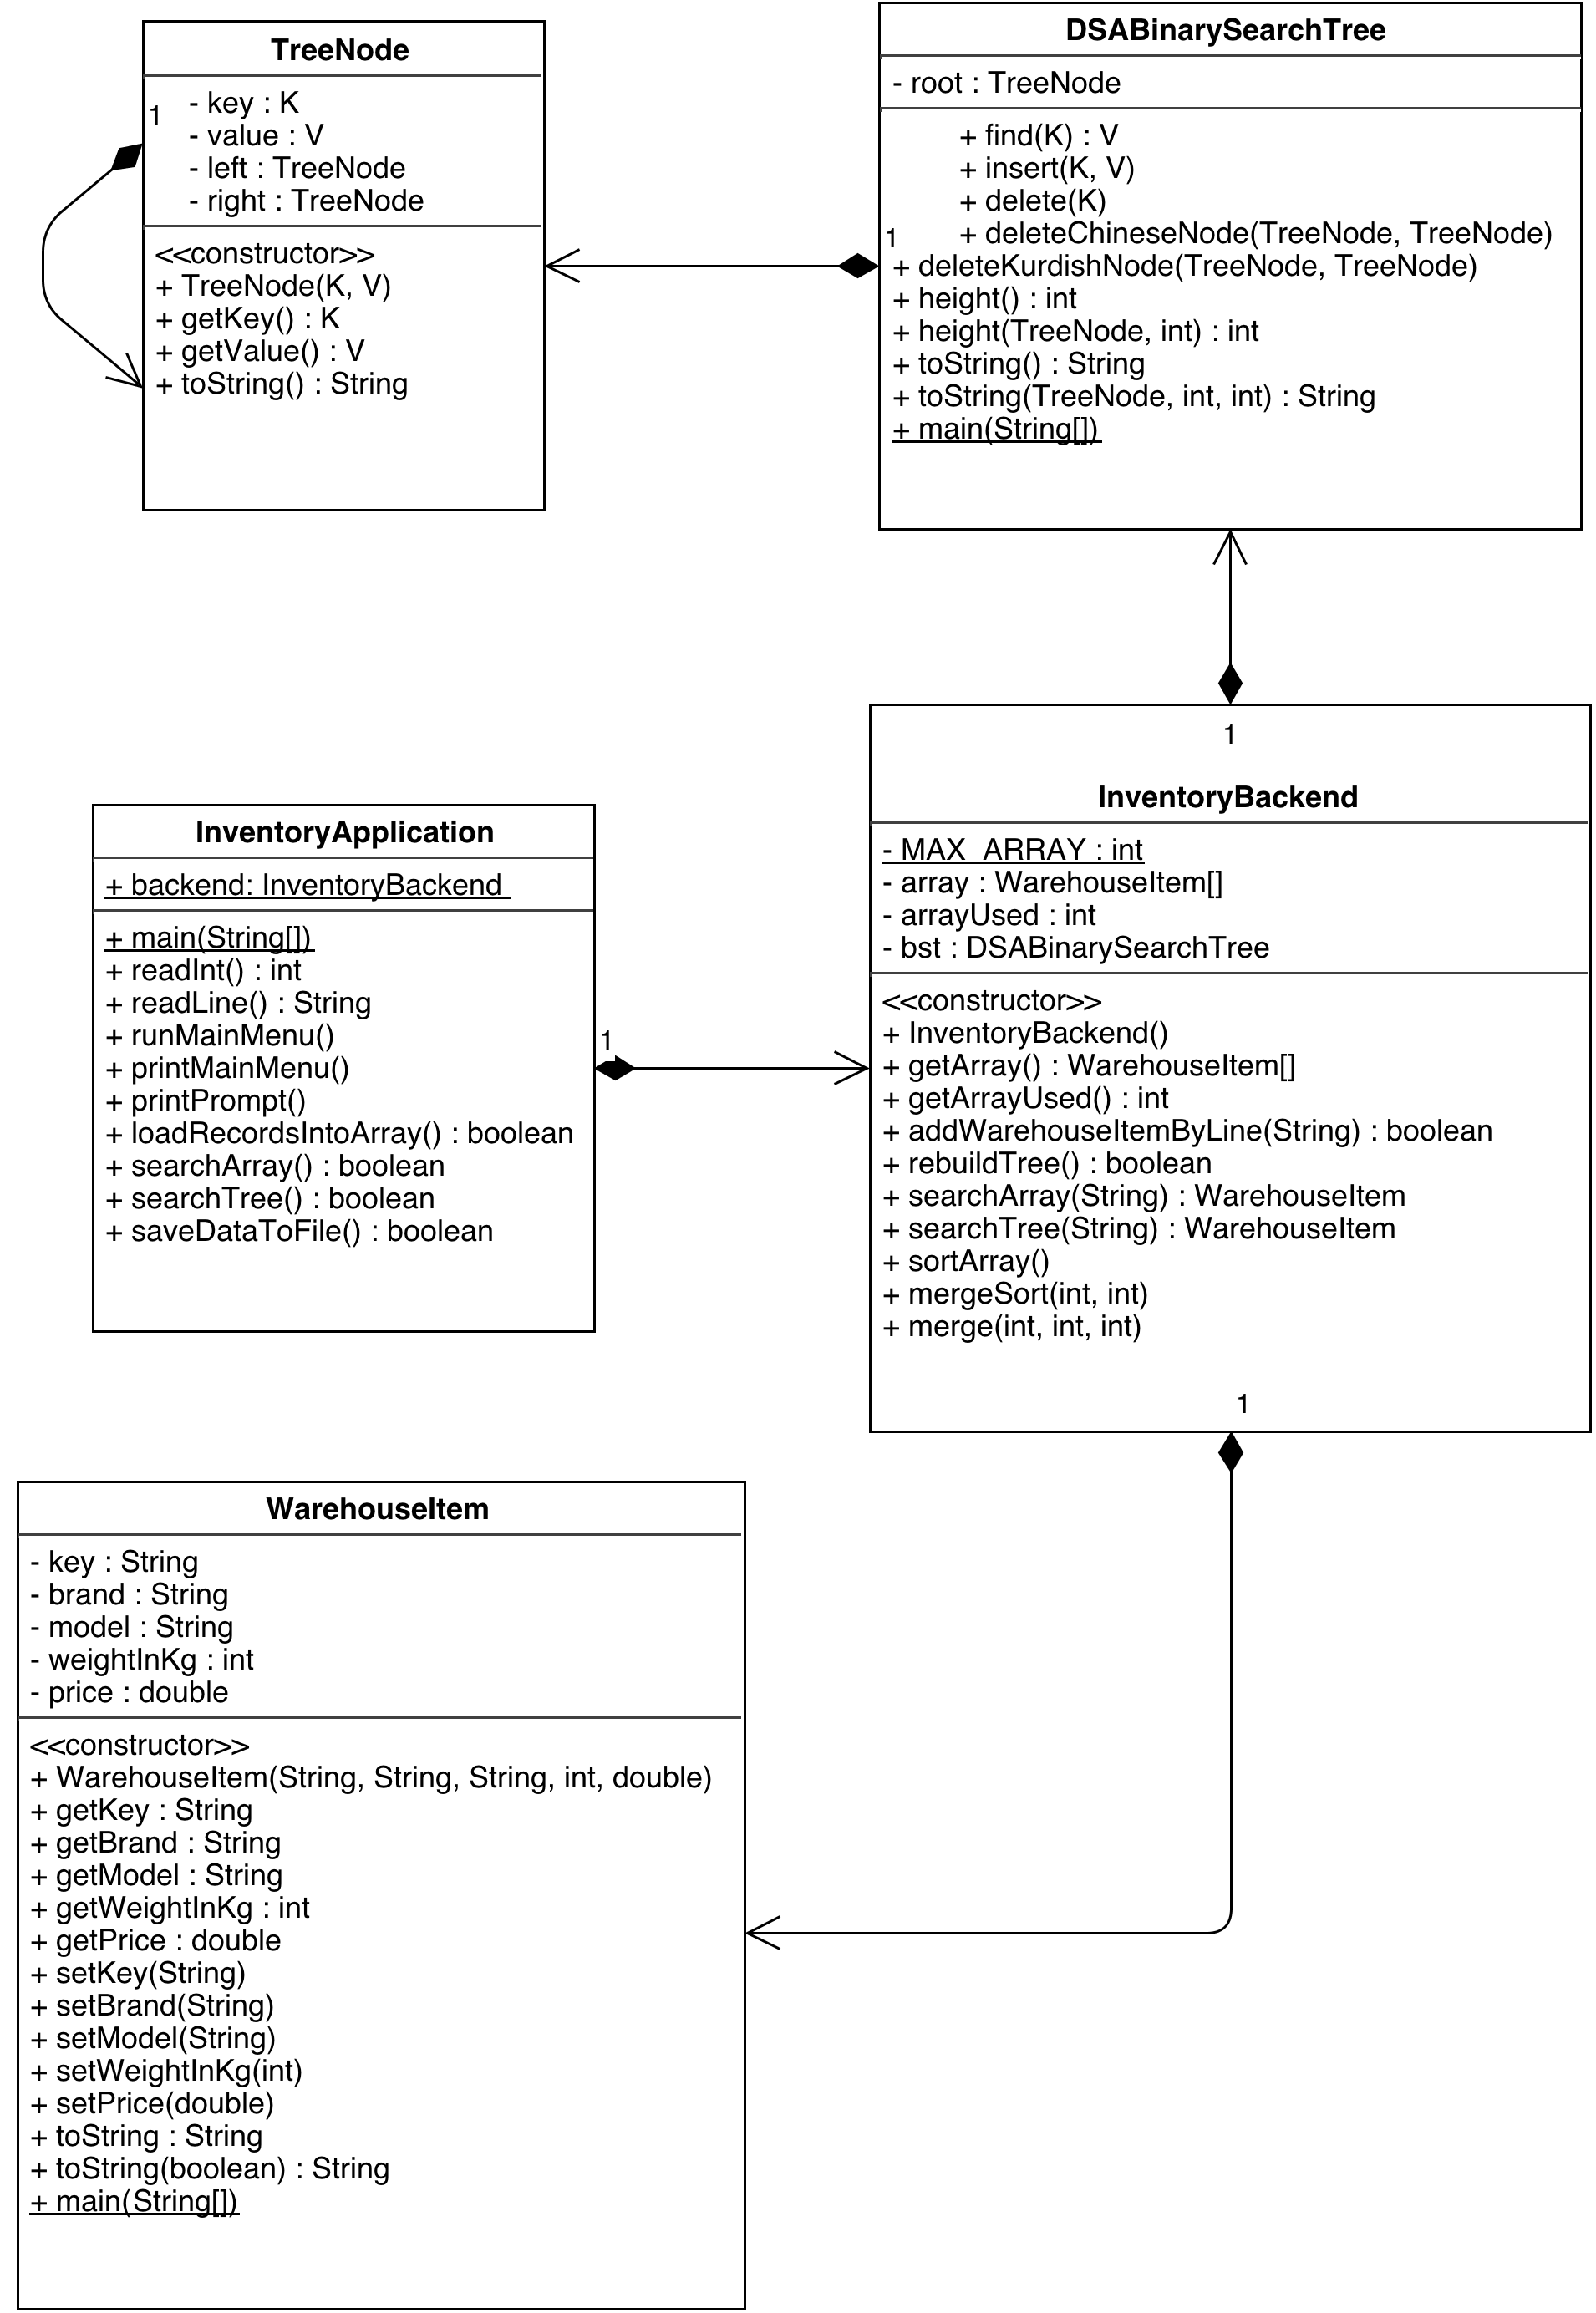
\includegraphics[width=15cm]{umldiagram.png}

\end{document}
